\section{Simulation Setup}

\begin{SCfigure}
	\centering
	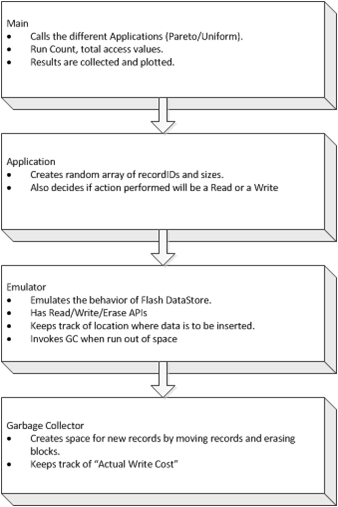
\includegraphics[width=0.4\textwidth]{C:/Ananth/OSU/CETI/MS-Thesis/MS-thesis-Report/imgs/Simulation-Flow-chart.png}
	\captionof{figure}{The {\bf Main} program controls the number of times the simulation is to be run and which application gets called among other things. It also collects the results returned by the {\bf Application} and generates the graphs. It invokes the {\bf Application} program which contains the implementation for Uniform, Pareto or BiModal type of distributions. Based on the toss of a coin, it decides if the next operation will be a read or a write. Every read and write operation invokes the {\bf Emulator} which contains functionalities such as reading/writing a record, maintaining the indices of the records within the Flash and so on. When space runs out, the {\bf Emulator} invokes the {\bf Garbage Collector} whose primary purpose is to free up space by moving around active records and erasing a block of inactive records. It is successful if it finds sufficient space for the next record to be inserted and it returns an exception back to the Emulator if it is not able to find space in the entire Flash.}
\end{SCfigure}


\subsection{Functions used in Simulator}

\begin{itemize}
\item {\bf Main}
\subitem {\emph runAppUniformDistribution(appRunCount)}
\subsubitem 	Arguments: appRunCount - Number of times the application is to be executed.
\subsubitem 	Return value: None
\subsubitem 	Functionality: Invokes the application.

\item {\bf Application}
\subitem {\emph AppUniformDistribution(seedVal,numOfRecords,RWAccessCnt,runIndex)}
\subsubitem 	Arguments: 	

\begin{tabbing}
	\= seedVal - Number of times the application is to be executed.\\
	\> numOfRecords - \\
	\> RWAccessCnt - \\
	\> runIndex - \\
\end{tabbing}

\subsubitem 	Return value: None
\subsubitem 	Functionality: Invokes the application.
 	
\end{itemize}

%-----------------------------------------------------------------------------------
\subsection*{Summary}
	Flash devices are making a great headway in becoming the storage device of choice in Mobile and Embedded systems. But they still have disadvantages such as a slow write speed which prevent them from being used as the primary storage device replacing RAMs. In order for them to perform optimally, Garbage Collectors are very important. This work analyzed the performance of five different GC algorithms against the most common of the traffic patterns in real-world applications (Uniform, Pareto and BiModal). The results that have come out of this study have gone against the existing results in current literature and hence have the potential to make rapid progress towards using Flash as primary storage. 

%-----------------------------------------------------------------------------------
\subsection*{Future work}
	

%-----------------------------------------------------------------------------------
\subsection*{Acknowledgements}
	I am grateful to Dr.Mukundan Sridharan who guided me during the course of this work. Thanks also to Dr.Rajiv Ramnath who during our weekly meetings, guided me in the right direction by asking lot of questions and helping me get the answers for them. My sincere gratitude also to Dr.Kenneth Parker and Dr.Anish Arora for giving me the opportunity to work on this wonderful project. Last but not the least, I am thankful to the professors and friends who helped me when I was stuck at a difficult problem. 